\documentclass[11pt]{article}
\usepackage[hmargin=1in,vmargin=1in]{geometry}
\usepackage{xcolor}
\usepackage{amsmath,amssymb,amsfonts,url,sectsty,framed,tcolorbox,framed,graphicx,bm}
\newcommand{\pf}{{\bf Proof: }}
\newtheorem{theorem}{Theorem}
\newtheorem{lemma}{Lemma}
\newtheorem{proposition}{Proposition}
\newtheorem{definition}{Definition}
\newtheorem{remark}{Remark}
\newcommand{\qed}{\hfill \rule{2mm}{2mm}}

\begin{document}
\noindent
\rule{\textwidth}{1pt}
\begin{center}
{\bf [CS304] Introduction to Cryptography and Network Security}
\end{center}
Course Instructor: Dr. Dibyendu Roy \hfill Winter 2022-2023 \\
Scribed by: Srushti Rathva (202051183) \hfill Lecture (Week 8-9) \\
\rule{\textwidth}{1pt}
\section*{Collision Finding Algorithm}
$h$ : $X \rightarrow Y$ \\
$|Y| = M$ \\\\
Choose any $X_{o} \subseteq X$ such that $|X_{o}| = Q$ \\
\hspace*{1.4cm}for each $x \in X_{o}$ \\
\hspace*{2cm}compute $y_{x} = h(x)$ \\
\hspace*{2cm}if $y_{x} = y_{x'}$ for some $x \neq x'$\\
\hspace*{2.5cm}return $(x,x')$ \\
\hspace*{2cm}else \\
\hspace*{2.5cm}return failure\\\\
$E_{i} :$ Event $h(x_{i}) \notin \{h(x_{1}),h(x_{2}),...,h(x_{i-1})\}$ \\
$X_{o} = \{x_{1},x_{2},...,x_{Q}\} \\\\$
\textbf{for i = 1}\\
$Pr[E_{1}] = 1 \\\\$
\textbf{for i = 2}\\
$Pr[E_{2} | E_{1}] = \frac{M-1}{M} \\\\
\frac{Pr[E_{1} \cap E_{2}]}{Pr[E_{1}]} = \frac{M-1}{M} \\\\
Pr[E_{1} \cap E_{2}] = \frac{M-1}{M} \times Pr[E_{1}] = \frac{M-1}{M} \\\\$
\textbf{for i = 3}\\
$Pr[E_{3} | E_{1} \cap E_{2}] =  \frac{M-2}{M} \\\\
\frac{Pr[E_{1} \cap E_{2} \cap E_{3}]}{Pr[E_{1} \cap E_{2}]} =  \frac{M-2}{M} \\\\
Pr[E_{1} \cap E_{2} \cap E_{3}] = \frac{M-2}{M} \times Pr[E_{1} \cap E_{2}] = \frac{M-2}{M} \times \frac{M-1}{M} \\\\$
\textbf{for i = 4}\\
$Pr[E_{4} | E_{1} \cap E_{2} \cap E_{3}] = \frac{M-3}{M} \\\\
\frac{Pr[E_{1} \cap E_{2} \cap E_{3} \cap E_{4}]}{Pr[E_{1} \cap E_{2} \cap E_{3}]} = \frac{M-3}{M} \\\\
Pr[E_{1} \cap E_{2} \cap E_{3} \cap E_{4}] = \frac{M-3}{M} \times Pr[E_{1} \cap E_{2} \cap E_{3}] = \frac{M-3}{M} \times \frac{M-2}{M} \times \frac{M-1}{M} \\\\ $
Continuing this process, \\
$Pr[E_{1} \cap E_{2} \cap E_{3} ... \cap E_{Q}] = \frac{M-1}{M} \times \frac{M-2}{M} \times \frac{M-3}{M} \times ... \times \frac{M-(Q-1)}{M} \\\\
Pr[Collision] = 1 - Pr[E_{1} \cap E_{2} \cap E_{3} ... \cap E_{Q}] \\\\
\hspace*{2cm} = 1 - [\frac{M-1}{M} \times \frac{M-2}{M} \times \frac{M-3}{M} \times ... \times \frac{M-(Q-1)}{M}] \\\\ 
\frac{M - i}{M} = 1 - \frac{i}{M} \approx e^{\frac{-i}{M}} \\
e^{-x} = 1 - x + \frac{x^{2}}{2!} - \frac{x^{3}}{3!} + ... \approx 1 - x \\
\\
\frac{M-1}{M} \times \frac{M-2}{M} \times \frac{M-3}{M} \times ... \times \frac{M-(Q-1)}{M} \approx  \Pi_{i=1}^{Q-1} e^{\frac{-i}{M}} \\\\
\hspace*{6cm} = e^{- \Sigma_{i=1}^{Q-1}\frac{i}{M}} \\\\
\hspace*{6cm} = e^{\frac{-1}{M}\Sigma_{i=1}^{Q-1}i} \\\\
\hspace*{6cm} = e^{\frac{-1}{M} \times \frac{(Q-1)Q}{2}} \\\\
Pr[Collision] \approx 1 - e^{\frac{-1}{M} \times \frac{(Q-1)Q}{2}} \\\\
\varepsilon \approx 1 - e^{\frac{-1}{M} \times \frac{(Q-1)Q}{2}} \\\\
1 - \varepsilon \approx  e^{\frac{-1}{M} \times \frac{(Q-1)Q}{2}} \\\\ $
Taking log on both sides \\\\
$ \frac{-(Q-1)Q}{2M} \approx ln(1-\varepsilon) \\\\
Q^{2} - Q \approx -2M \times ln(1-\varepsilon) \\\\
Q^{2} - Q \approx 2M \times ln(\frac{1}{1-\varepsilon}) \\\\
Q^{2} \approx 2M \times ln(\frac{1}{1-\varepsilon}) \\\\
Q \approx \sqrt{2M \times ln(\frac{1}{1-\varepsilon})}  \\\\ $
For $\varepsilon = 0.5$, \\\\
$Q \approx \sqrt{2M \times ln(\frac{1}{1-0.5})} \\\\
\hspace*{0.3cm} \approx 1.177 \sqrt{M} \\\\ $
For $\varepsilon = 0.9$, \\\\
$Q \approx \sqrt{2M \times ln(\frac{1}{1-0.9})} \\\\
\hspace*{0.3cm} \approx 2.14 \sqrt{M} \\\\ 
Q = O(\sqrt{M}) \\$
Hence, the complexity of finding collision is = $O(\sqrt{M})$ \\\\
\textbf{Summary} \\
$h : X \rightarrow Y \hspace*{2cm} |Y| \leq 2|X|$ \\
Time Complexity of Preimage Finding Algorithm = $O(|Y|)$ \\
Time Complexity of Second Preimage Finding Algorithm = $O(|Y|)$ \\
Time Complexity of Collision Finding Algorithm = $O(\sqrt{|Y|})$ \\\\
$h : \{0,1\}^{*} \rightarrow \{0,1\}^{m}$ \\
where, h is secure hash function \\
Time Complexity of Preimage Finding Algorithm = $O(2^{m})$ \\
Time Complexity of Second Preimage Finding Algorithm = $O(2^{m})$ \\
Time Complexity of Collision Finding Algorithm = $O(2^{m/2})$ 

\section*{Compression Function}
$h : \{0,1\}^{m+t} \rightarrow \{0,1\}^{m}$ \\\\
\textbf{Target : } \\
Construct $ H : \{0,1\}^{m+t} \rightarrow \{0,1\}^{m}$ from $h$. \\
Security of $H$ will completely depend on security of $h$. \\\\
Given, $x \in \{0,1\}^{*}$ \\
\hspace*{1.2cm}$|x| = $ length of $x$ \\
\hspace*{1.2cm}$|x| \geq m+t+1 $ \\\\
From $x$ construct a $y$ such that, \\
$|y| \equiv$ 0(mod t) \\\\
The absolute value of $ y $ is defined :
\[ y = \begin{cases}
x & \mbox{if $|x| \equiv$ 0(mod t) } \\
x || 0^{d} & \mbox{if $|x| + d \equiv$ 0(mod t)}\\
\end{cases}
\] 
Select IV : $\{0,1\}^{m}$ \\
$ y = y_{1} || y_{2} || ... || y_{r}$ \\
Such that, $|y_{i}| = t \hspace*{1cm} 1 \leq i \leq r$ \\\\
\begin{center}
$ H = 
\begin{cases}
Z_{0} = IV \\
Z_{1} = h(Z_{0} || y_{1}) \\ 
Z_{2} = h(Z_{1} || y_{2}) \\
\vdots \\
Z_{r} = h(Z_{r-1} || y_{r}) 
\end{cases} $
\end{center}
$
x' = Z_{r-1} || y_{r} \\
|x'| = m + t \\
IV = Z_{r-1} \\\\
x^{*} = y_{r} \\
x'_{1} = Z^{1}_{r-1} || y^{1}_{r} \\
x'_{2} = Z^{2}_{r-1} || y^{2}_{r} \\\\
h(x'_{1}) = h(x'_{2}) \\
H(x'_{1}) = H(x'_{2}) $

\subsection*{Length Extension Attack } 
$ M = y_{1} || y_{2} || ... || y_{r} \\\\
Z_{r} = h(Z_{r-1} || y_{r}) \\ $
where, \\
$ Z_{i} = h(Z_{i-1} || y_{i}) \hspace*{1cm} 1 \leq i \leq r \\
Z_{0} = IV $ \\\\
Given $(M,Z_{r})$ is it possible to find $(M_{2},Z_{r})$ without computing H on $(M_{2},Z_{r})$. \\\\
$M_{2} = M || y_{r+1} \hspace*{3cm} |y_{t+1}| = t $\\
$h(Z_{r} || y_{r+1}) = Z   \hspace*{2.7cm} H(M) = Z_{r}$\\

\subsection*{Merkle-Damgard Principle}
Compress : 
$: \{0,1\}^{m+t} \rightarrow \{0,1\}^{m}  \hspace*{2cm} t \geq 2 \\\\
n = |x| \\
k = \lceil \frac{n}{t-1} \rceil \\
d = k(t-1) - n $ \\\\
for i = 1 to k-1 \\
$y_{i} = x_{i}$ \\
$y_{k} = x_{k} || 0^{d}$ \\
$y_{k+1}$ = binary(d) \\
$Z_{1} = 0^{m+1} || y_{1} \\
g_{1} = $ compress($Z_{1}$) \\
for i=1 to k-1 \\
\hspace*{0.5cm} $Z_{i+1} = g_{i} || 1 || y_{i+1}$ \\
\hspace*{0.5cm} $g_{i+1} = $ compress($Z_{i+1}$) \\
$h(x) = g_{k+1} \\$ 
return $h(x)$ \\

\section*{Secure Hash Algorithm (SHA)}
1. SHA - 160 \\
2. SHA - 256 \\
3. SHA - 512 \\

\subsection*{SHA-I}
$ |x| \leq 2^{64} -1 \\
d = (447 - |x|) $ mod 512 \\
$l = $ binary($|x|$) \\
$ y = x || 1 || 0^{d} || l $ \\
$ |y| = |x| + 1 + d + |l| \equiv 0$ (mod 512) \\\\
\textbf{ROTL$^{S}$(X)} \\
Circular left shift on X by S position. \\\\
$ \textbf{$\bm{f_{t}(B,C,D)}$} = 
\begin{cases}
(B \wedge C) \vee ((\neg B) \vee D)  \hspace*{2cm}0 \leq t \leq 19 \\
B \oplus C \oplus D \hspace*{3.8cm}20 \leq t \leq 39 \\
(B \wedge C) \vee (B \vee D) \vee (C \vee D) \hspace*{0.8cm}40 \leq t \leq 59 \\
B \oplus C \oplus D \hspace*{3.8cm}60 \leq t \leq 79 \\
\end{cases} $ \\\\\\
$y$ = SHA-I-PAD($x$) \\
$ y = M_{1} || M_{2} || ... || M_{n} \hspace*{2cm} |M_{i}| = 512$ \\\\
$ 
H_{0} = 67452301 \\
H_{1} = EFCDAB89 \\
H_{2} = 98BADCFE \\
H_{3} = 10325476 \\
H_{4} = C3D2E1F0 \\\\
k_{t} =
\begin{cases}
5A827999 \hspace*{2cm}0 \leq t \leq 19 \\
6ED9EBA1 \hspace*{1.5cm}20 \leq t \leq 39 \\
8F1BBCDC \hspace*{1.4cm}40 \leq t \leq 59 \\
CA62C1D6 \hspace*{1.7cm}60 \leq t \leq 79 \\
\end{cases} $ \\\\\\
for i=1 to n \\
$M_{i} = w_{0} || w_{1} || w_{2} || ... || w_{15}$ \hspace*{2cm} $w_{i}$ =32 \\
for t=16 to 79 \\
\hspace*{0.5cm}$w_{t} = ROTL^{1}(w_{t-3} \oplus w_{t-8} \oplus w_{t-14} \oplus w_{t-16)} $ \\
$
\hspace*{0.5cm} A = H_{0} \\ 
\hspace*{0.5cm} B = H_{1} \\ 
\hspace*{0.5cm} C = H_{2} \\ 
\hspace*{0.5cm} D = H_{3} \\ 
\hspace*{0.5cm} E = H_{4} \\
$
for i=0 to 79 \\
$
\hspace*{0.5cm}temp = ROTL^{5}(A) + f_{k}(B,C,D) + E + w_{t} + k_{t} \\
\hspace*{0.5cm} E = D \\ 
\hspace*{0.5cm} D = C \\ 
\hspace*{0.5cm} C = ROTL^{30}(B) \\ 
\hspace*{0.5cm} D = A \\ 
\hspace*{0.5cm} E = temp \\
H_{0} = H_{0} + A \\
H_{1} = H_{1} + B \\
H_{2} = H_{2} + C \\
H_{3} = H_{3} + D \\
H_{4} = H_{4} + E \\$
return ($(H_{0} || H_{1} || H_{2} || H_{3} || H_{4})$)

\section*{Message Authentication Code (MAC)}
\textbf{Alice} \hspace{6.5cm} \textbf{Bob} \\
$C = E(M,K)\xrightarrow{\hspace*{2.5cm}C\hspace*{2.5cm}} \sim C$ \\
$MAC = h(M,K)\xrightarrow{\hspace*{2cm}MAC\hspace*{2cm}} \sim MAC$ \\\\
$Dec( \sim C,K) = \sim M \\
h(\sim M, K) = MAC_{1} \\ $
If $ \sim MAC = MAC_{1} \\ $
then accept $\sim M$ as $\sim M = M $

\section*{Hash based Message Authentication Code (HMAC)}
ipad = 363636 ... $\rightarrow$ 512 bits \\
opad = 5c5c5c ... $\rightarrow$ 512 bits \\
K $\rightarrow$ secret key \\
SHA $\rightarrow$ SHA - I \\
$HMAC_{K}(x) = SHA((K \oplus opad)) || SHA((K \oplus ipad) || x) $

\section*{CBC - Message Authentication Code (MAC)}
$ x = (x_{0} || x_{1} || x_{2} || x_{3} || ... || x_{n})$ \\
IV = 00...0 \\
$y_{0} = $IV \\
for i=1 to n \\
\hspace*{0.5cm} $y_{i} = Enc((y_{i-1} \oplus x_{i}),K)$ \\
return $y_{n}$

\section*{One Time Padding (OTP)}
$C = M \oplus K \\
len(K) \geq len(M) \\
C_{1} = M_{1} \oplus K \\
C_{2} = M_{2} \oplus K $ \\
OTP is not practical. \\\\
\textbf{F(K,IV)} = $Z_{i}$ \\
K $\rightarrow$ Secret key \\
IV $\rightarrow$ Initialisation vector (Public)\\\\
$
\hspace*{0.65cm} Z_{0} \hspace*{0.25cm} Z_{1} \hspace*{0.25cm} ... \hspace*{0.25cm} Z_{n-1} \\
\oplus \hspace*{0.25cm} m_{0} \hspace*{0.25cm} m_{1} \hspace*{0.25cm} ... \hspace*{0.25cm} m_{n-1} \\
\hspace*{0.65cm} \overline{c_{0} \hspace*{0.40cm} c_{1} \hspace*{0.40cm} ... \hspace*{0.40cm} c_{n-1}} 
$ \\\\
\textbf{Properties}\\
1. $Z_{0},Z_{1} ... Z_{n-1}$ will be a randomly looking string. \\
2. If the same input (K,IV) is given to the function in different time, it will generate same output $Z_{i}$ \\
3. If K is generated randomly and kept secret then the outputs $Z_{0},Z_{1} ... Z_{n-1}$ will be indistinguishable from bits strings generated by a random bit generator. \\
4. F is Pseudorandom bit generator. \\
5. Length of the output bits $>>>$ length of K. \\
\hspace*{1cm}If K $\rightarrow$ 80 bits then,\\
\hspace*{1cm}We can encrypt $2^{80} - 1$ large number and $Z_{i}$ will repeat almost after $2^{80} - 1$ numbers.\\
6. If we modify atleast one bit of IV or K then there will be an unpredictable change in the output $Z_{i}$. \\

\section*{Stream Cipher}
Encryption is done bitwise \\
There are two types of stream cipher : \\
1. Synchronous \\ 2. Asynchronous

\subsection*{Synchronous Stream Cipher}
Plaintext and Ciphertext are not involved in key generation. \\
State update function : $S_{i+1} = f(S_{i},K)$ \\
Keystream generator function : $Z_{i} = g(S_{i},K)$ \\
Ciphertext generator function : $c_{i} = h(Z_{i},m_{i})$ \\
$S_{0}$ is generated from $K$ and $IV$.

\subsection*{Asynchronous Stream Cipher}
Plaintext and Ciphertext are involved in key generation. \\
State update function : $\sigma_{i+1} = f(\sigma _{i},K,IV)$ \\
Keystream generator function : $Z_{i} = g(\sigma _{i},K)$ \\
Ciphertext generator function : $c_{i} = h(Z_{i},m_{i})$ \\

\subsection*{Linear Feedback Shift Register (LFSR)}
$S_{i} \in \{0,1\} \hspace*{2cm} 0 \leq i \leq n-1$ \\
t $ \rightarrow$ clocking number \\\\
t = 0 \\
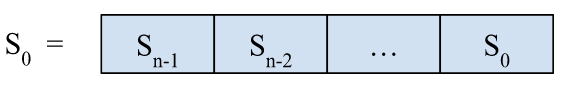
\includegraphics[width=200pt]{p1.png} \\\\
t = 1 \\
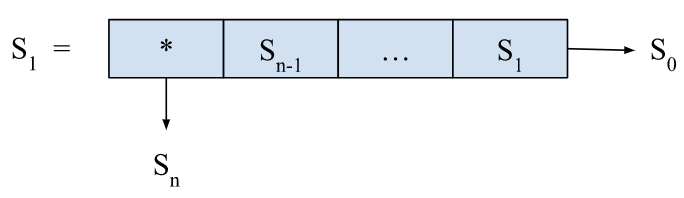
\includegraphics[width=240pt]{p2.png} \\
t = 2 \\
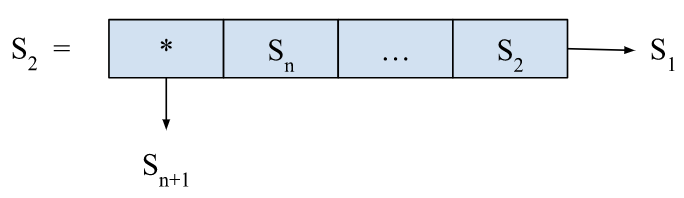
\includegraphics[width=240pt]{p3.png} \\
The escaping bit is the Output and additional bits on the left are called Feedback bits. \\
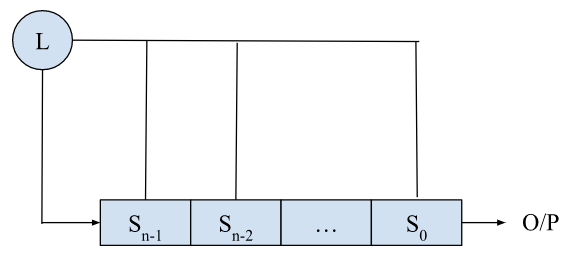
\includegraphics[width=250pt]{p4.png} \\
$L(S_{0},S_{1},..,S_{n-1}) = S_{n} \in \{0,1\}$ \\
$L : \{0,1\}^{n} \rightarrow \{0,1\}$ \\
$L_{a} = a_{0}S_{0} \oplus a_{1}S_{1} \oplus ... \oplus a_{n-1}S_{n-1}$ \\
$a_{i} \in \{0,1\}$ \\\\
\textbf{Period of LFSR} \\
$S_{0} \rightarrow$ Non zero initial state \\
$S_{0}$ will be repeated after m clocking of LFSR then m is called period of LFSR. \\
$L = S_{0} \oplus S_{1}$ \hspace*{1cm}(3 bits LFSR) \\
Period = $2^{3} - 1 = 7$\\\\
\textbf{Full Periodic LFSR} \\
An n-bit LFSR will be called full periodic LFSR if period of the LFSR is $2^{n}-1$. \\
Period of LFSR is completely dependent on the linear feedback function. \\\\\\
Consider an n bit LFSR,\\
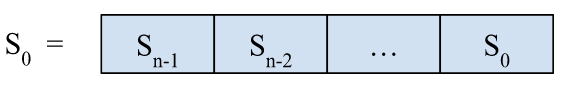
\includegraphics[width=200pt]{p1.png} \\
$S_{n} = L(S_{0},...,S_{n-1}) \\
\hspace*{0.5cm} = c_{1}S_{n-1} \oplus c_{2}S_{n-2} ... \oplus c_{n}S_{0}\\\\
S_{n+1} = L(S_{1},...,S_{n})\\$
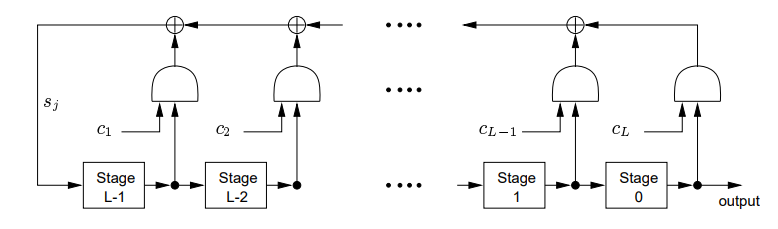
\includegraphics[width=400pt]{p5.png} \\
$L = c_{1}S_{n-1} \oplus c_{2}S_{n-1}... \oplus c_{n}S_{0}\\
f(x) = 1 + c_{1}x + c_{2}x^{2} +....+ c_{n}x^{n}\\
f(x) \in F2[x] \hspace{1cm} c_{i} \in {0,1}\\\\ $
n bit LFSR $\longleftrightarrow$ Liner feedback function $\longleftrightarrow$ polynomial of degree $\leq$ n in F2[x]\\\\
\textbf{Properties}\\
1. If the connection polynomial or feedback polynomial is primitive polynomial then the corresponding LFSR will have full period.\\
For n-bit LFSR period will be 2$^n$ -1.\\
2. If the polynomial is irreducible then the period of the LFSR will divide 2$^{n}$ - 1.\\
3. If it is reducible then different state will have different cycle length or different period.\\\\
Consider n bit LFSR,\\
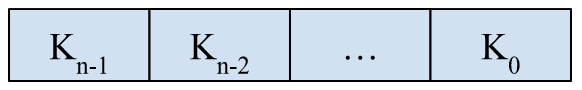
\includegraphics[width=200pt]{p6.png}\\
$K = (K_{0},K_{1},...,K_{n-1})$\\
Output bits $x_{i} \rightarrow $ Keystream bits $Z_{i}$ \\
$m_{i} \oplus Z_{i} = c_{i} \rightarrow$ Ciphertext \\\\
\textbf{Known Plaintext attack}\\
$Z_{i} = m_{i} \oplus c_{i} \hspace{1cm} 0 \leq i \leq n-1$ \\
$Z_{0} = K_{0},Z_{1} = K_{1},...,Z_{n-1} = K_{n-1}$ \\\\
If we are given keystream bits then we'll be able to prepare a system of linear equations. By solving these equations we'll get back the state.\\\\
Suppose $Z_{i}$ are the outputs from function $f$\\
 $Z_{i} \in \{0,1\} \\
 c_{i} = m_{i} \oplus Z_{i}$\\
 State update of LFSR :\\
 1) Linear feedback\\
 2) Shifting\\
 State update function of LFSR is : $\alpha$\\
 $S_{t+1} = \alpha(S_{t}) \\
 Z_{t+1} = f(S_{t+1}) $ \\\\
 $ 
\begin{bmatrix}
S^{t+1}_{0}\\
S^{t+1}_{1}\\
.\\
S^{t+1}{n-1}
\end{bmatrix}
=
\begin{bmatrix}
0 & 1 & .. & .. & .. & 0\\
0 & 0 & 1 & .. & .. & 0\\
0 & 0 & 0 & 1  & .. & 0\\
0 & 0 & 0 & .. & .. & 1\\
\end{bmatrix}
\begin{bmatrix}
S^{t}_{0}\\
S^{t}_{1}\\
.\\
S^{t}_{n-1}
\end{bmatrix}\\\\
L = C_{n-1}S_{0} \oplus C_{n-2}S_{1} \oplus .... \oplus C_{0}S_{n-1}$\\\\
\textbf{Non linear LFSR with combination functions}\\
$f: \{0,1\}^{l} \rightarrow \{0,1\}$ \\
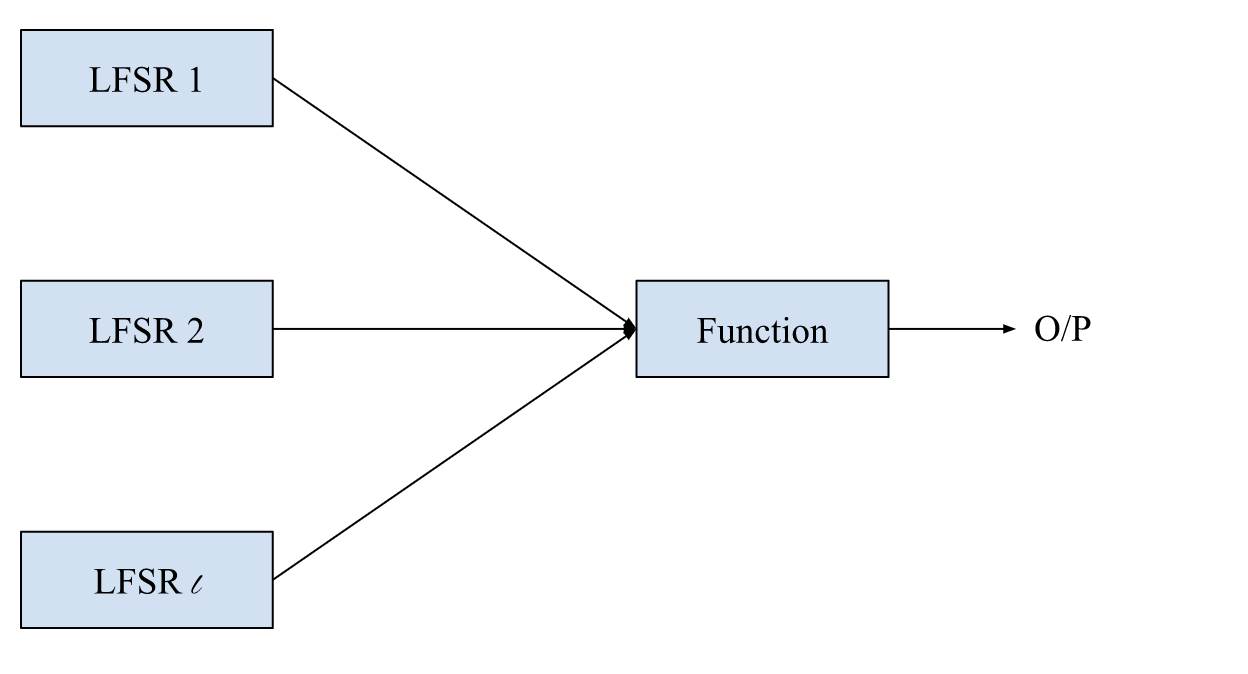
\includegraphics[width=350pt]{p7.png} \\\\
\textbf{Non linear feedback bit shift register (NFSR)}\\
Feedback function is non-linear. \\
\end{document}
